\chapter{Kerr-Newman black holes with scalar hair}
\label{ch:KN}

\epigraph{``\emph{
Bræður munu berjast \\
og að bönum verðast, \\
munu systrungar \\
sifjum spilla; \\
hart er í heimi, \\
hórdómur mikill, \\
skeggöld, skálmöld, \\
skildir eru klofnir, \\
vindöld, vargöld, \\
áður veröld steypist, \\
mun engi maður \\
öðrum þyrma. 
} 
''}{44th verse of Völuspá}


\section{Introduction}

It is to be expected that KBHsSH, just like the Kerr solution, admit electrically charged generalizations.
The astrophysical interest of such solutions is, perhaps, more limited due to efficient discharge mechanisms, but understanding their existence and their physical properties is of relevance to fully grasp the impact of this scalar (or other) hair on the paradigmatic BHs of General Relativity.
In addition to this, the Kerr-Newman solution introduces some interesting features to the rotating black hole spacetime.
Namely, a energy and angular momentum component \emph{outside} the horizon and a dipole magnetic moment induced by the rotating electric charge.
The corresponding gyromagnetic ratio turns out to have precisely the non-anomalous electron value, $g=2$.

In this chapter we will show that this is the case and to this end, we will first consider an ungauged scalar field around a Kerr-Newman black hole.
The domain of these solutions is bounded by uncharged boson stars and as such, no new soliton solutions arise.
However, after achieving this, we will also study a gauged scalar field around a Kerr-Newman black holes and there the solitonic limit is electrically charged.
Due to this, we will also construct electrically charged rotating boson stars.

%%%%%%%%%%%%%%%%%%%%%%%%%%%%%%%%
\section{The ungauged scalar field model}
\label{sec_mod_u}
%%%%%%%%%%%%%%%%%%%%%%%%%%%%%%%%
%%%%%%%%%%%%%%%%%%%%%%%%%%%%%%%%
\subsection{Action, equations of motion and ansatz}
\label{sec_mofrl}
%%%%%%%%%%%%%%%%%%%%%%%%%%%%%%%%
We start by considering Einstein-Maxwell theory, minimally coupled to a complex, massive (mass $\mu$)  ungauged scalar field $\Psi$, whose action is given by
%
\begin{eqnarray}
  \label{KNaction}
 \mathcal{S} = \frac{1}{4\pi G}\int d^4x \sqrt{-g}\left[\frac{R}{4}- \frac{1}{4}F_{ab}F^{ab}- g^{ab}\Psi^*_{,a}\Psi_{,b} -\mu^2\Psi^*\Psi \right]\ ,  
\end{eqnarray}  
where $F_{ab}$ are the components of the Maxwell 2-form, $F$, related to the 1-form potential $A=A_adx^a$ as $F=dA$. The Einstein-Klein-Gordon-Maxwell equations, obtained by varying the action with respect to the metric, scalar field and electromagnetic field, are, respectively,
%
%
\begin{equation}
G_{ab}  = 2\left( T_{ab}^\Psi+T_{ab} ^{\rm EM} \right)\ , \qquad \Box \Psi =\mu^2\Psi \ , \qquad D_aF^a_{~b}=0 \ ,
\label{KNeom}
\end{equation}
where the two components of the energy-momentum tensor are
%
\begin{equation}
\label{KNemt}
T_{ab}^\Psi \equiv  
 \Psi_{ , a}^*\Psi_{,b}
+\Psi_{,b}^*\Psi_{,a} 
-g_{ab}  \left[ \frac{1}{2} g^{cd} 
 ( \Psi_{,c}^*\Psi_{,d}+
\Psi_{,d}^*\Psi_{,c} )+\mu^2 \Psi^*\Psi\right] \ , \qquad
 T_{ab}^{\rm EM} \equiv F_a^{~c}F_{bc} - \frac{1}{4}g_{ab}F_{cd}F^{cd} \ .
\end{equation}
This model is invariant under a \textit{global} transformation $\Psi\rightarrow \Psi e^{i\alpha}$, where $\alpha$ is constant.



Kerr-Newman black holes with ungauged scalar hair (KNBHsUSH) are obtained using the metric and scalar field given by Eqs. \eqref{eqn:HBH-ansatz} and \eqref{eqn:field-ansatz}, and the electromagnetic potential ansatz is
%
\begin{align}
 \label{electric_ansatz}
 A_adx^a &= \left( A_t - A_\varphi W\sin\theta \right)dt + A_\varphi\sin\theta d\varphi \ ,
\end{align}
where $A_t$ and $A_\varphi$, depend only on the spheroidal coordinates $r$ and $\theta$ just as the metric and scalar field functions.
As in the previous chapters, we shall focus on nodeless $m=1$ solutions as an illustrative case.

%%%%%%%%%%%%%%%%%%%%%%%%%%%%%%%%
\subsection{Boundary conditions}
\label{KNBCs}
% %%%%%%%%%%%%%%%%%%%%%%%%%%%%%%%%
In order to find Kerr-Newman black holes with ungauged scalar hair, we must impose boundary conditions.
In addition to the boundary conditions described in Appendix \ref{BCs} for KBHsSH, we require that at spatial infinity
\begin{equation}
  \lim_{r\rightarrow\infty}A_\varphi=\lim_{r\rightarrow\infty}A_t=0\ .
\end{equation}
Observe that the last equality could be changed to a constant, rather than zero, in a different gauge.

On the symmetry axis, $i.e.$ at $\theta=0,\pi$, axial symmetry and regularity require that
\begin{equation}
  \label{ABCs}
  \partial_\theta A_t = \phi = A_\varphi = 0\ .
\end{equation} 
% %
By writing an approximate form of the solution near the horizon as a power series in the coordinate $x=\sqrt{r^2-r_H^2}$, we find
\begin{equation}
  A_t \big|_{x=0} =  \Phi_H,~~ \partial_x A_\varphi \big|_{x=0}=0 ,
\end{equation}
where $\Phi_H$ is the horizon electrostatic potential. 
%
%
% %%%%%%%%%%%%%%%%%%%%%%%%%%%%%%%%
\subsection{Physical quantities}
% \label{sec_pq}
% %%%%%%%%%%%%%%%%%%%%%%%%%%%%%%%%
% These quantities can be split into the horizon contribution -- computed as a Komar integral on the horizon -- and the matter contributions, composed of the scalar field and electromagnetic parts, computed as the volume integrals of the appropriate energy-momentum tensor components: 
% %
The contribution of the electromagnetic field changes some of the physical quantities described in Appendix \ref{BCs}.
Namely, each equation in Eq. \eqref{MH-hor} obtains a new contribution from the electromagnetic field
\begin{eqnarray}
  \label{KNMH-hor}
  M=M^\Psi+M^{\rm EM}+M_H\ , \qquad J=J^\Psi+J^{\rm EM}+J_H\ ,
\end{eqnarray}
where $M^{\rm EM}$ and $J^{\rm EM}$ are the mass and angular momentum contributions of the electromagnetic field respectively.
The solutions possess an electric charge $Q_E$ that can be computed using Gauss's law, 
on any closed 2-surface covering the horizon. 
Alternatively, $Q_E$ can be computed from the decay of the 4-potential, together with the magnetic dipole moment $\mu_M$:
 \begin{eqnarray}
 \label{asym-matter-fields}
  A_t\sim 
  \frac{Q_E}{r}+\dots \ , \qquad A_{\varphi}\sim \frac{\mu_M \sin \theta}{r}+\dots\
   .
 \end{eqnarray}
As with the Kerr-Newman black holes, the gyromagnetic ratio $g$ defines how the magnetic dipole moment 
is induced by the total angular momentum and charge, for a given total mass:
\begin{equation}
  \mu_M=g\frac{Q_E}{2M}J \ .
  \label{gyro}
\end{equation}
The Smarr mass formula obtains an additional term
%
\begin{eqnarray}
  \label{KNsmarr}
  M=2 T_H S +2\Omega_H (J-m Q) + \Phi_H Q_E+ M^\Psi,
\end{eqnarray}
and so does the first law
\begin{eqnarray}
\label{first-lawKN}
dM=T_H dS +\Omega_H dJ + \Phi_H dQ_E\ .
\end{eqnarray}
Finally, observe that relations \eqref{KNsmarr} and \eqref{KNMH-hor} are consistent with a different Smarr relation, only in terms of horizon quantities  

\begin{eqnarray} 
  M_H=2T_H S+2 \Omega_H J_H~,
% + \Phi_H Q_E \ .
\end{eqnarray}
together with the electromagnetic relation $M^{\rm EM}=\Phi_HQ_E+2\Omega_HJ^{\rm EM}$.

%%%%%%%%%%%%%%%%%%%%%%%%%%%%%%%%%%%%%%%%%%%%
\subsection{Results }
\label{sec_results_u}
%%%%%%%%%%%%%%%%%%%%%%%%%%%%%%%%%%%%%%%%%%%%
% As in the previous work \cite{Herdeiro:2015gia,Herdeiro:2016tmi} and previous chapters of this essay
% the numerical integration is performed with 
% dimensionless variables introduced by using natural units set by $\mu$ and $G$.
% The global charges and all other quantities of interest are also
%  expressed in units set by $\mu$ and $G$ 
% (we set $G=1$ in what follows). 
% In particular this means we set $\mu Q_E\rightarrow Q_E$; 
% note that $\Phi_H$ is dimensionless (in units such that $4\pi \epsilon_0=1$). 

In order to obtain an overview of the domain of existence of KNBHsUSH we have to fix the new degree of freedom, related to electric charge. 
As was briefly mentioned above, similarly to the
KN case, no solitonic limit exists, for a nonzero $Q_E$.
Thus, for most of the numerical solutions we have chosen to fix the electrostatic potential on the horizon $\Phi_H$
and vary the remaining  input parameters $w$ and $r_H$.
This allows these  two-dimensional sections of the full domain of existence to reach the solitonic limit, 
wherein the horizon area vanishes and the electrostatic potential becomes constant everywhere and pure gauge.


 In Fig.~\ref{fig:w-M} (left panel), 
we exhibit the $(\Omega_H,M)$ domain of existence of the solutions, where we have fixed the horizon electrostatic potential to be $\Phi_H=0.3$. Observe that the domain therein was obtained by extrapolating into the continuum
the results from discrete sets of around two thousand numerical solutions; we also remark that a qualitatively similar picture has been found for $\Phi_H=0.6$.
 As shown in the main panel (the inset is for $\Phi_H=0$), 
this domain of existence is bounded by boson stars (red solid line), 
the KN limit (blue dotted line -- dubbed \textit{existence line}) 
and the extremal KNBHsUSH limit (green dashed line). 
The last two limits vary with the electrostatic potential whereas the first one does not; 
this can be observed in the right panel, where part of the line of extremal KNBHsUSH is shown for $\Phi_H=0$, $0.6$ and $0.8$, as well as the corresponding existence line and extremal Kerr-Newman BHs (black solid lines). 
The trend is that the larger the electrostatic potential becomes, the lower the mass of the extremal Kerr-Newman BH is, along the existence line (henceforth dubbed as \textit{Hod point}, following~\cite{Herdeiro:2015tia}), whence the line of extremal KNBHsUSH starts. This is the expected result from the known behaviour of Kerr-Newman BHs. Another trend, illustrated by comparing the main left panel with the inset, is that for higher $\Phi_H$, there are extremal hairy BHs with lower horizon angular velocity.
Note that the maximal frequency of extremal KNBHsUSH increases as can be seen from the right panel of Fig. \ref{fig:w-M}.

%%%%%%%%%%%%%%%%%%%%%%%%%%%%%%%%%%%%%%%%%%%%%%%%%%%%%%%%%%%%%%%%%%%%%%%%%%
\begin{figure}[h!]
  \begin{center}
    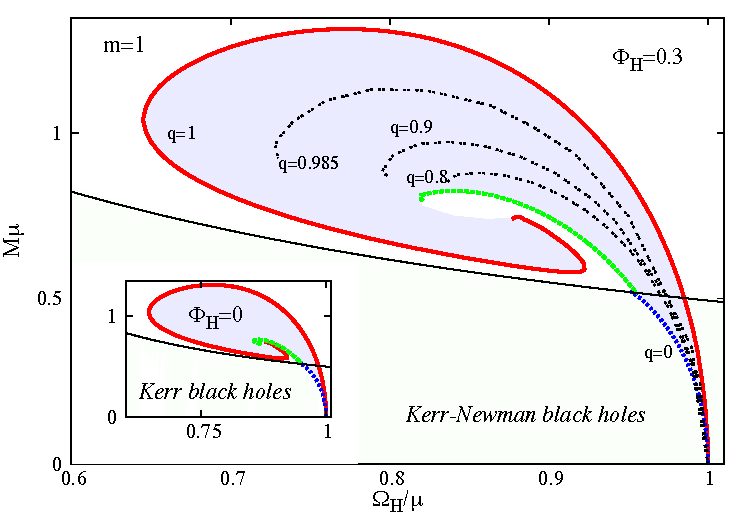
\includegraphics[width=0.48\textwidth]{papers/KerrNewman/BH-w-M} 
    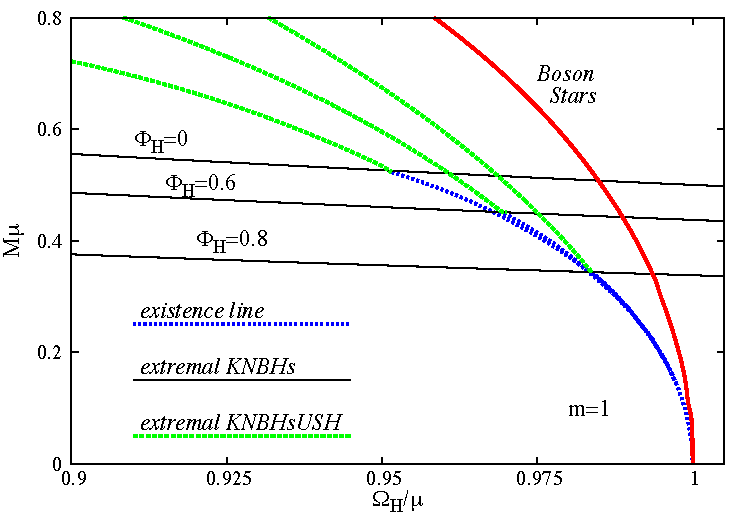
\includegraphics[width=0.48\textwidth]{papers/KerrNewman/zoom-w-M}
  \end{center}
  \caption{The $(\Omega_H,M)$ domain of existence for a sample of KNBHsUSH. (Main left panel) Diagram for $\Phi_H=0.3$ with the boson star envelope (red solid line), the existence line on the domain of KN BHs (blue dotted line) and the line of extremal KNBHsUSH (green dashed line). The black solid line corresponds to the extremal KN BHs; non-extremal solutions exist below. The black dotted lines have constant normalized Noether charge $q$. (Inset) diagram for $\Phi_H=0$, for comparison. (Right panel) Detail around the intersection of the existence lines with the extremal KNBHsUSH lines and the extremal KN lines for $\Phi_H=0,0.6$ and $0.8$.  
	}
  \label{fig:w-M}
\end{figure}
%%%%%%%%%%%%%%%%%%%%%%%%%%%%%%%%%%%%%%%%%%%%%%%%%%%%%%%%%%%
 
  
 In Fig.~\ref{fig:w-g} (left panel), we exhibit the ratio $ M^{\Psi}/M$, which gives another measure of hairiness
   as a function of $\Omega_H$,
for $\Phi_H=0.3$. The figure shows that small fractions of the total energy in the hair are only allowed for sufficiently large horizon angular velocity. When the angular velocity is small, equilibrium between the hair and the horizon is only possible for solutions with $q$ close to unity, $i.e.$ boson star-like. 
The inset in this figure shows the $(\Omega_H,Q_E)$ domain of existence of the KNBHsUSH solutions. It illustrates that the electric charge of the solutions, for fixed $\Omega_H$ between that of the Hod point and the maximum allowed frequency, $\Omega_H=\mu$, is maximized along the existence line (and in particular at the Hod point). But for lower values of the frequency, slightly larger charges than that found at the Hod point are possible, occurring along the extremal hairy BHs line.

%%%%%%%%%%%%%%%%%%%%%%%%%%%%%%%%%%%%%%
\subsubsection{Gyromagnetic ratio}
%%%%%%%%%%%%%%%%%%%%%%%%%%%%%%%%%%%%%%
Rotating charges give rise to a magnetic dipole moment, $\mu_M$. 
In classical electromagnetism, a generic relation of the form~\eqref{gyro}, 
between $\mu_M$ and the total angular momentum, mass and charge can be derived, 
for systems with constant ratio of charge to mass density, yielding $g=1$. 
When experiments such as that performed for Stern and Gerlach in the early 20th century, 
showed that the electron should have $g=2$, it became clear that a new fundamental description 
for the electron was necessary, beyond the scope of the non-relativistic quantum theory. 
Such a description appeared with the Dirac equation, which, from first principles predicts $g=2$, 
a value that is corrected by loop diagrams in Quantum Electrodynamics (QED), 
yielding the so called anomalous magnetic moment, whose agreement 
with experiment is one of the outstanding successes of QED.

In BH physics, Carter first observed that $g=2$ for the KN solution. 
Since then many other studies considered the gyromagnetic ratio of rotating charged BHs, 
for instance with different asymptotics and in higher dimensions (see $e.g.$~
\cite{Garfinkle:1990ib,Herdeiro:2000ap,Aliev:2004ec,Ortaggio:2006ng,Aliev:2006tt}). 
Here we show that the addition of scalar hair leads to a suppression of the gyromagnetic ratio, 
and of the corresponding magnetic dipole moment, 
with respect to that of a comparable KN BH.  
 A novel aspect is that $g$ 
can be smaller than 1, a rather unsual feature in other models of relativistic, 
charged and spinning compact objects, 
$cf.$~\cite{Novak:2003uj}. 


In Fig.~\ref{fig:w-g} (right panel), we exhibit the gyromagnetic ratio in a $(q,g)$-diagram, for KNBHsUSH with $\Phi_H=0.3$.
The diagram shows that the gyromagnetic ratio, $g$, of both the extremal and non-extremal hairy BH solutions, is always less than $2$.
As expected, it does approach $2$, for both cases, in the limit of vanishing hair.
Further insight is obtained by considering the quantity
\begin{align}
\Delta\equiv \frac{M^2}{Q_E^2+J^2/M^2} \ ,
\end{align}
which determines the KN bound $\Delta\geqslant 1$. Indeed, all KN BHs have $\Delta>1$. This bound is, however, violated by a large set of KNBHsUSH, in particular by those close to the BS limit. This is reminiscent of what has been found for KBHsSH - see the discussions in~\cite{Herdeiro:2014goa,Herdeiro:2015gia,Herdeiro:2015tia,Delgado:2016zxv}.  Our results show that
solutions with $g<1$ predominantly exhibit $\Delta<1$ and thus violate the KN bound -- $cf.$ the inset of Fig.~\ref{fig:w-g} (right panel).



%%%%%%%%%%%%%%%%%%%%%%%%%%%%%%%%%%%%%%%%%%%%
\begin{figure}[H]
  \begin{center}
    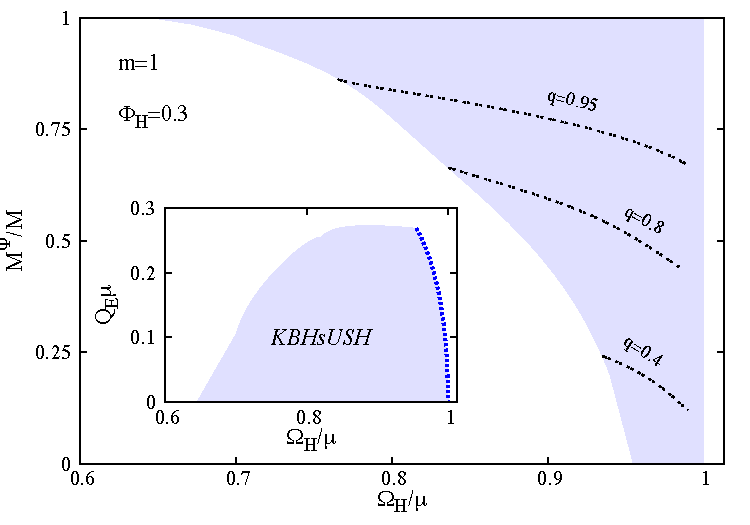
\includegraphics[width=0.48\textwidth]{papers/KerrNewman/Mpsi}
    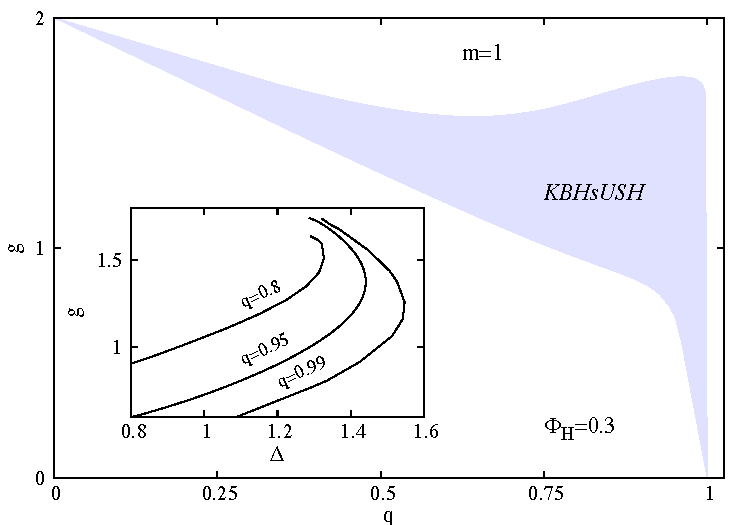
\includegraphics[width=0.48\textwidth]{papers/KerrNewman/qg}
  \end{center}
  \caption{(Left panel) The ratio $M^\Psi/M$ is shown as a function of $\Omega_H$ for a sample of KNBHsUSH. The inset shows the electric charge as a function of $\Omega_H$, where the blue dotted line is the existence line. 
	(Right panel)  The $(q,g)$ space. The inset show $g$ as a function of $\Delta$, that determines the KN bound.
}
\label{fig:w-g} 
\end{figure}
%%%%%%%%%%%%%%%%%%%%%%%%%%%%%%%%%%%%%%%%%%%%

 
 


%%%%%%%%%%%%%%%%%%%%%%%%%%%%%%%%%%%%%%%%%%%%
\section{Gauged scalar field model}
\label{sec_mod_g}
%%%%%%%%%%%%%%%%%%%%%%%%%%%%%%%%%%%%%%%%%%%%




%%%%%%%%%%%%%%%%%%%%%%%%%%%%%%%%
\subsection{Main differences in the model}

%%%%%%%%%%%%%%%%%%%%%%%%%%%%%%%%

Let us now consider the model described in Section~\ref{sec_mod_u} but with a \textit{gauged} scalar field, 
that couples minimally to the electromagnetic field, with gauge coupling $q_E$. 
This coupling is implemented by replacing the partial derivatives of the scalar field in the action~\eqref{KNaction} as
\begin{equation}
\partial_a \Psi \longrightarrow D_a\Psi=\partial_a \Psi + iq_E A_a \Psi \ .
\label{KNmc}
\end{equation}
The Einstein equations still take the form~\eqref{KNeom}, but with the substitution~\eqref{KNmc} 
in the scalar field energy-momentum tensor~\eqref{KNemt}. Then, the scalar and Maxwell equations of motion become
\begin{eqnarray}
\label{field-eqs}
D_{a}D^{a}\Psi=\mu^2 \Psi\ , \qquad 
\nabla_{b}F^{ba}=
iq_E \big [ (D^{a}\Psi^*) \Psi-\Psi^*(D^a \Psi) \big ] 
\equiv q_E j^a  \ .
\end{eqnarray}  
Physically, the scalar field is now electrically charged, 
and its quanta, the scalar particles, carry a charge $q_E$.
Thus the scalar field sources the Maxwell field.

This model is invariant under the $local$ U(1) gauge transformation 
\begin{eqnarray}
\label{gauge-transf}
\Psi \to \Psi e^{-i q_E \alpha}\ ,~~A_a\to A_a+\partial_a \alpha \ ,
\end{eqnarray}
where $\alpha$ is a real function. One consequence of this gauge invariance is that the $(t, \varphi)$-dependence of the scalar field ansatz~\eqref{eqn:field-ansatz}, 
can now be gauged away by applying the local $U(1)$ symmetry
(\ref{gauge-transf})
with $\alpha =  (m\varphi -w t)/q_E$.  This, however, also changes the gauge field, as $A_t\to A_t-w/q_E$,
$A_\varphi \to A_\varphi+m/q_E$. 
%
Consequently, the solutions cannot be constructed starting with the configurations in the
previous sections and increasing $q_E$.
%
Thus, in order
to be able to consider this approach, we  keep the $(t,\varphi)$-dependence in 
the scalar field ansatz and fix the corresponding gauge freedom by setting $A_t = A_\varphi = 0$ at infinity.

One major difference with respect to the case 
discussed in the previous section 
 is that the solitonic limit of the solutions carries now a nonzero electric charge.
Self-gravitating charged boson stars were first considered, in spherical symmetry, in~\cite{Jetzer:1989av} 
(see also the recent work  \cite{Pugliese:2013gsa}). 
To the best of our knowledge, no rotating generalizations of these static solutions have been reported\footnote{ 
Some properties of the spinning charged solitons, 
with a self-interacting ($Q$-ball type) scalar field model, were addressed in~\cite{Brihaye:2009dx}.
}.
The Noether charge $Q$ of the solitons, $i.e.$ the total
particle number, is now intrinsically related to the electric charge $Q_E$. 
The former can be computed as  
%
\begin{eqnarray}
\label{Q1}
Q= \int j^t \sqrt{-g} dr  d\theta d\varphi=
 4\pi \int_{0}^\infty dr \int_0^\pi d\theta  
~r^2\sin \theta ~e^{-F_0+2F_1+F_2}  (w-q_E A_t -mW)\phi^2 \ ,
\end{eqnarray}
%
whereas the latter is read from the asymptotics
 of the electric potential $A_t$, as given by Eq. \eqref{asym-matter-fields}.
A straightforward computation 
shows that both the Noether charge and the electric charge of the spinning \textit{solitons}
are proportional  to the total angular momentum,
\begin{eqnarray}
\label{JQ}
J= m Q=\frac{4 \pi m Q_E}{q_E}\ .
\end{eqnarray} 


%%%%%%%%%%%%%%%%%%%%%%%%%%%%%%%%%%%%%%%%%%%%%%%%%%%%%%%%%%%%%%%%%%
\subsection{Features of the gauged scalar field solutions}
\label{sec_results_g}
%%%%%%%%%%%%%%%%%%%%%%%%%%%%%%%%%%%%%%%%%%%%%%%%%%%%%%%%%%%%%%%%%%
 
The construction of the  gauged scalar field solutions is similar 
to that described above for the ungauged case ($q_E=0$ limit).
In particular, the KNBHsGSH are subject to the same set of 
boundary conditions  used in the ungauged case.
The synchronization condition, however, is different,   
\begin{equation}
\label{cond-new}
 w-q_E \Phi_H=m \Omega_H \ ,
\end{equation}
in agreement with the result found in the linear theory~\cite{Hod:2014baa,Benone:2014ssa}.

As mentioned in the introduction to this chapter, the electrically charged boson stars form a part of the domain of existence of KNBHsGSH. 
Thus we have paid special attention to this limiting case.
These solutions  are obtained by considering the ansatz~\eqref{eqn:HBH-ansatz}--\eqref{electric_ansatz} with $r_H=0$ 
and replacing the boundary conditions at the horizon,~\eqref{bch1} and \eqref{ABCs},
by the following boundary conditions at the origin
\begin{eqnarray}
\label{bc0} 
\partial_r F_i|_{r=0}= 
W|_{r=0}=0\ ,~~
\phi| _{r =0}=0\ ,~~\partial_r A_t|_{r=0}=A_\varphi|_{r=0}=0\ .
\end{eqnarray}
% 

Some results of the numerical integration are shown in Fig.~\ref{fig:w-M-gauged} (left panel).
The basic properties of the spinning gauged boson stars solutions can be summarized as follows.
First, for all values of the gauge coupling considered so far, 
the frequency dependence of the solutions is qualitatively similar to the ungauged case.
The solutions 
exist for a limited range of frequencies
$0<w_{min}<w<\mu$. 
In particular, we observe that the minimal frequency increases with $q_E$. 
After this minimal frequency, a backbending towards larger values of $w$ occurs, yielding a second branch of solutions. 
A second backbending, towards
smaller values of $w$,  is observed as the frequency reaches a maximal value along the second branch, $w\to w^{\rm 2nd}_{\rm max}$, whose value increases again with $q_E$. 
Then, similarly to the ungauged limit, a third branch of solutions develops -- not shown in Fig.~\ref{fig:w-M-gauged} (left panel).
Subsequently, we expect the existence of an inspiraling behaviour of the solutions, 
in analogy with uncharged boson stars, towards a limiting configuration.  


%%%%%%%%%%%%%%%%%%%%%%%%%%%%%%%%%%%%%%%%%%%%%%%%%%%%%%%%%%%
\begin{figure}[H]
  \begin{center}
    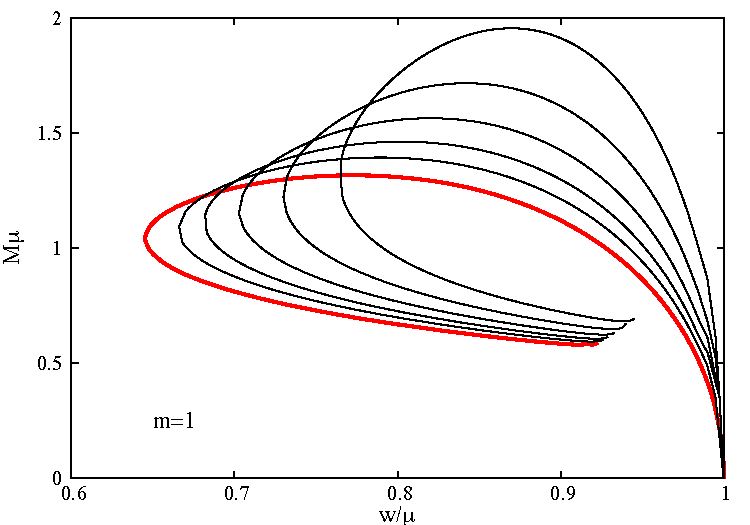
\includegraphics[width=0.48\textwidth]{papers/KerrNewman/BS-w-M-gauged}
    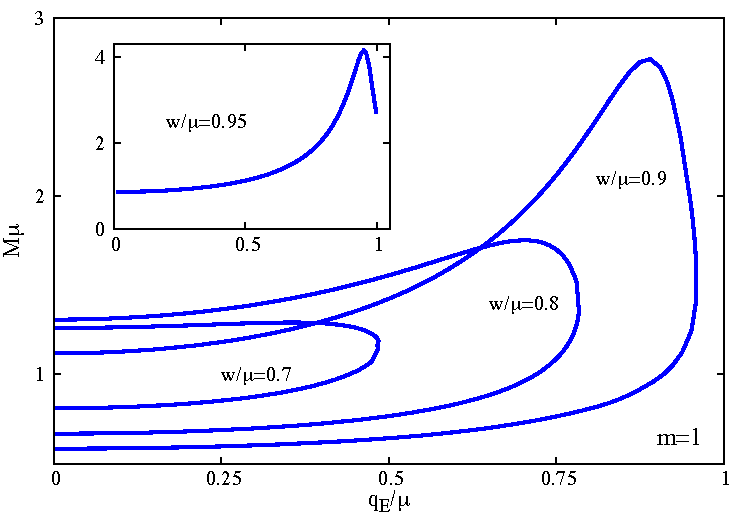
\includegraphics[width=0.48\textwidth]{papers/KerrNewman/BS-g-M-gauged}
  \end{center}
  \caption{
	(Left panel)
	The $(w,M)$ diagram for spinning boson stars with $q_E=0$ (red curve), $q_E/\mu=0.2, 0.3, 0.4, 0.5$
	and $0.6$ (top curve).  
		(Right panel)
	The mass $M$ is shown as a function of the gauge coupling constant $q_E$
	for several frequencies, $w/\mu=0.7, 0.8, 0.9$ and $0.95$ (as an inset).	}
  \label{fig:w-M-gauged}
\end{figure}
 %%%%%%%%%%%%%%%%%%%%%%%%%%%%%%%%%%%%%%%%%%%%%%%%%%%%%%%%%%%
Although only the mass is displayed in Fig.~\ref{fig:w-M-gauged} (left panel), the $J(w)$
diagram has a very similar shape.
Consequently,  the axially symmetric gauged boson stars do not possess
a static limit.  Observe also that the maximal mass of spinning gauged boson stars solutions increases with $q_E$.

As shown in Fig.~\ref{fig:w-M-gauged} (right panel), 
the solutions possess also a nontrivial dependence on 
the gauge coupling constant $q_E$.
For given values of $w$,
spinning solutions exist up to a maximal
value of the gauge coupling constant only, $q_E=(q_E)_{max}$.
The physical rationale behind this behaviour 
is similar to that discussed for the spherically symmetric case 
\cite{Jetzer:1989av,Pugliese:2013gsa}.
For $q_E>(q_E)_{max}$ the charge repulsion  becomes bigger than
  the scalar and gravitational attraction and localized solutions cease to exist  
(note that the maximal value of $q_E$
increases with frequency).
Also, as seen in Fig.~\ref{fig:w-M-gauged} (right panel),
all global charges stay finite as $q_E\to (q_E)_{max}$.

\bigskip

KNBHsGSH are obtained by adding a horizon at the center of the spinning gauged boson star  
we have just described, which can be done for  any such  solution.
One way to construct the BHs
  is to  start from  boson stars 
and slightly increase the horizon size via the parameter $r_H$.
In this approach, the other input parameters 
$\Omega_H$, $q_E$,  $\Phi_H$ and $m$
are kept fixed. 
We recall that for BHs, the frequency $w$ is fixed by the synchronization condition (\ref{cond-new}).
Then one finds three 
possible behaviours for
the resulting branches of BH solutions -- see Fig.~\ref{fig:q-AH-gauged} (left panel).
($i$) First, for small enough values of $\Omega_H$,
 the branch of BHs connects two different boson stars; 
as $r_H\to 0$ the horizon area vanishes, $q\to 1$, while the temperature
 diverges.
($ii$) For intermediate values of  $\Omega_H$,
the branch of solutions ends in an extremal KNBHsGSH solution. 
These limiting configurations have finite
horizon size   and global charges, $0<q<1$ and appear to possess 
a regular horizon.
($iii$) Finally, for large values of $\Omega_H$,
the branch of  KNBHsGSH interpolates between 
a charged boson star and a set of critical KN solutions (with $q=0$ and $A_H>0$), which lie again 
on an {\it existence line}. 

 In Fig.~\ref{fig:q-AH-gauged} (right panel) we exhibit the (Komar) energy density and angular momentum density (in the inset) for an illustrative example of a KNBHGSH  with physical input parameters 
$r_H=0.24$, $w =0.86$, $q_E =0.2$, $\Phi_H=0.1$. 
These densities have a contribution from both the electromagnetic and the scalar field. The main feature we wish to emphasize is the composite structure revealed by the plots. KN BHs have an (electromagnetic) energy and angular momentum density that decays with the radial coordinate, whereas KBHsSH 
(and boson stars)
have toroidal-like distributions for the (scalar) energy and angular momentum densities. 
Consequently, KNBHsGSH exhibit a superposition of these two behaviours, with decaying densities from the horizon but which exhibit a local maximum, in the neighbourhood of the equatorial plane, at some finite radial coordinate. 
A similar energy and angular momentum distribution can be found for KNBHsUSH.  

The behaviours illustrated in Fig.~\ref{fig:q-AH-gauged} supports the expectation that the domain of existence of KNBHsGSH will fill in the domain delimited by the boson star curves exhibited in Fig.~\ref{fig:w-M-gauged} (left panel), together with the existence line of KN BHs and a line of extremal KNBHsGSH,  in a qualitatively similar fashion to that shown in Fig.~\ref{fig:w-M} (left panel). Having established these solutions exist, and that their domain of existence will be analogue to the case of KNBHsUSH, we will not enter further details here.
Here we mention only that, similar to the ungauged case, 
the gyromagnetic ratio of  KNBHsGSH constructed so far is always smaller than $g=2$.


%%%%%%%%%%%%%%%%%%%%%%%%%%%%%%%%%%%%%%%%%%%%%%%%%%%%%%%%%%%
\begin{figure}[H]
  \begin{center}
    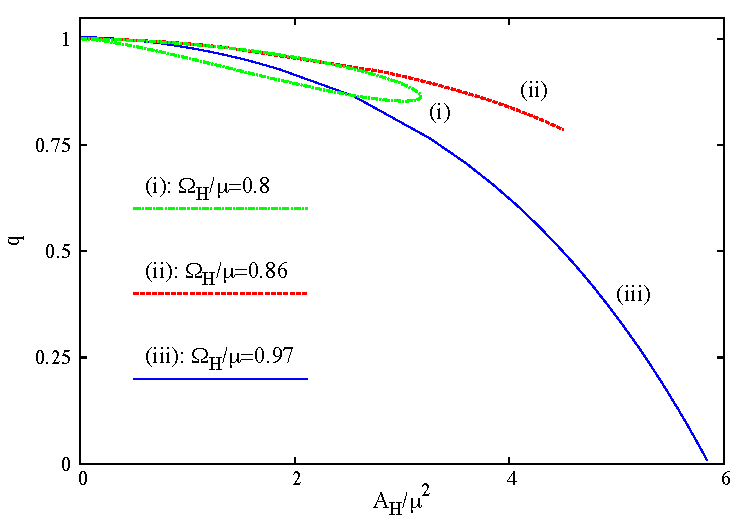
\includegraphics[width=0.48\textwidth]{papers/KerrNewman/BH-q-AH} 
    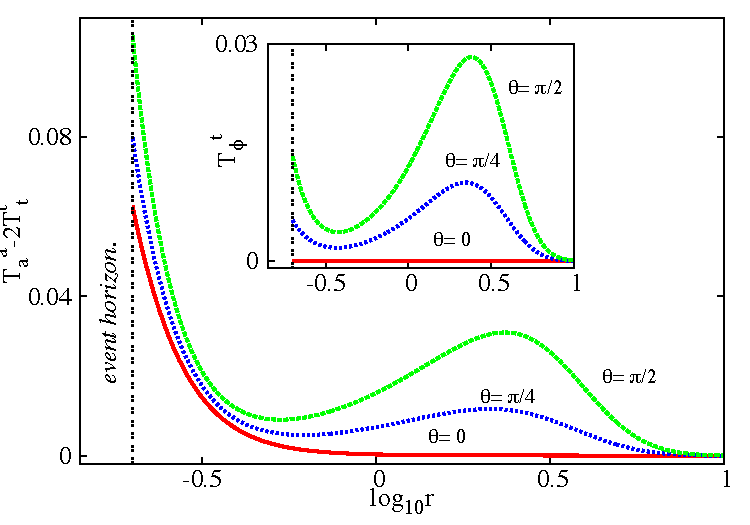
\includegraphics[width=0.48\textwidth]{papers/KerrNewman/energy-2d} 
  \end{center}
  \caption{ (Left panel) 
	The $(A_H,q)$ diagram is shown for three sets of KNBHsGSH solutions with fixed values of 
$\Omega_H$ and 
$q_E/\mu=0.2$, 
$\Phi_H=0.1$. (Right panel) 
 Energy density (and angular momentum density in the inset) along three different slices of constant $\theta$ for an illustrative example of a KNBHGSH.
	}
  \label{fig:q-AH-gauged}
\end{figure}
 %%%%%%%%%%%%%%%%%%%%%%%%%%%%%%%%%%%%%%%%%%%%%%%%%%%%%%%%%%%
 


%%%%%%%%%%%%%%%%%%%%%%
\section{Discussion}
\label{sec_remarks}
%%%%%%%%%%%%%%%%%%%%%%%

% The Kerr solution~\cite{Kerr:1963ud}, which describes the paradigmatic BH geometry in General Relativity, allows a generalization with electric (or magnetic) charge~\cite{Newman:1965my}, discovered shortly after the Kerr metric. Much more recently, it was found that the Kerr solution also allows a generalizations with scalar~\cite{Herdeiro:2014goa,Herdeiro:2015gia,Kleihaus:2015iea,Herdeiro:2015tia,Chodosh:2015oma} or Proca hair~\cite{Herdeiro:2016tmi}. The former are known as Kerr BHs with scalar hair (KBHsSH).
In this chapter we showed that electric charge can be added to KBHsSH, both considering an ungauged and a gauged scalar field and analysed some basic properties of the solutions.
In both cases, their domain of existence is qualitatively similar to the of the uncharged hairy BHs.
In particular it is bounded by three curves, corresponding do the solitonic limit (boson stars), extremal hairy BHs, and bald (KN) BHs.
In the gauged case, the solitonic limit corresponds to rotating charged boson stars, which until now had not been studied in the literature. 

These results indicate that by adding scalar hair to the electrically charged Kerr-Newman blackhole suppresses some of the electromagnetic properties of the black hole.
As an example of this we have considered the gyromagnetic ratio, $g$, and found that it is always lower than the well known the relativistic (Dirac) value for Kerr-Newman black holes, $g=2$~\cite{Carter:1968rr}, only reaching the limit when the hair vanishes.

There are other interesting applications for these solutions such as testing the no-short-hair conjecture.
This will be discussed further in Chapter \ref{ch:conclusions}.
